%----------------------------------------------------------
%	PACKAGES AND THEMES
%----------------------------------------------------------
\documentclass[aspectratio=169,xcolor=dvipsnames,handout]{beamer}

\usetheme{Darmstadt}
\usecolortheme{seahorse}
\usepackage[hangul]{kotex}
\usepackage{hyperref}
\usepackage{graphicx, array, adjustbox}
\usepackage{booktabs, multicol, multirow}
\setbeamercovered{transparent}

%----------------------------------------------------------
%	TITLE PAGE
%----------------------------------------------------------

\title[]{고용관계에 대하여} % The short title appears at the bottom of every slide, the full title is only on the title page
\subtitle{노사관계의 이론과 실제}
\author[]{오성재}
\institute[CNU] % Your institution as it will appear on the bottom of every slide, may be shorthand to save space
{
    충남대학교 경제학과\\
}
\date{2024년 9월 4일} % Date, can be changed to a custom date

\begin{document}

\begin{frame}
    \titlepage
\end{frame}

\begin{frame}{목차}
    \tableofcontents[hideallsubsections]
\end{frame}

\section{고용관계의 배경}

\begin{frame}{산업사회와 노동문제}
    \begin{itemize}
        \item 노동문제(특히 파업)는 사용자와 노동자간의 노사관계가 존재하는 상황에서 항상 발생 가능한 현상임
        \begin{itemize}
            \item 최초의 파업: 고대 이집트 피라미드 건설 근로자 파업
            \item 자본주의나 공산주의 체제와 상관없이 노사관계 존재
        \end{itemize}
        \item 17세기 말 산업혁명 이후 노동조합 조직 시작
        \item 산업혁명은 급속한 경제발전 및 취업구조의 변화 촉발
        \begin{itemize}
            \item 가내수공업에서 제조업 중심으로 산업구조 변화
            \item 임금노동자 비율의 증가가 노동운동 촉발
            \item 20세기 후반까지 제조업 중심의 노사관계
        \end{itemize}
    \end{itemize}
\end{frame}

\begin{frame}
    \begin{figure}
        \centering
        \includegraphics[width=.95\textwidth]{pic/연도벌 사업별 취업자 비율.png}
        \\
        \raggedright % 왼쪽 정렬
        \hspace{1em} % 좌측 여백을 추가
        \tiny{자료 : 통계청(2021)} % 자료 출처
        \caption{연도별 산업별 취업자 비율}
    \end{figure}
    \begin{itemize}
        \item 한국을 포함한 자본주의 사회에서 제조업 비중 감소, 서비스업 비중 증가
        \item 서비스업의 고용관계 중요성 증대
    \end{itemize}
\end{frame}

\subsection{정보화$\cdot$세계화와 고용관계}

\begin{frame}{정보화와 세계화}
    \begin{itemize}
        \item 20세기 말부터 정보화와 세계화는 무한경쟁을 유도하고 이는 새로운 형태의 노사갈등 촉발
        \begin{itemize}
            \item 정보화 : 인터넷(WWW)과 개인용 컴퓨터(PC)의 보급
            \item 세계화 : 개별 사건의 파장이 지구촌 전체에 영향을 줌
        \end{itemize}
    \end{itemize}
\end{frame}

\begin{frame}{정보화와 세계화 시대의 고용관계}
    \begin{itemize}
        \item 정보화와 세계화에 의한 극한경쟁의 시대 도래 :
        \begin{itemize}
            \item 생존을 위한 생산적$\cdot$협조적 고용관계의 정립 여부가 국가 경쟁력을 좌우
        \end{itemize}
        \item 새로운 형태의 노사갈등의 탄생 :
        \begin{itemize}
            \item 비정규직 양산, 구조조정의 상시화 등 인적자원의 유연화로 근로자의 고용불안이 커지고 있음
            \item 특수고용직(청년유니온, 학교비정규직노조, 라이더유니온)의 등장 및 증가
        \end{itemize}
    \end{itemize}
\end{frame}

\subsection{4차 산업혁명$\cdot$고용관계}

\begin{frame}{}
    \begin{itemize}
        \item 인공지능(AI)로 대표되는 4차산업혁명 시대의 도래.
        \begin{itemize}
            \item 신 기술 도입에 의한 노동시장의 급격한 변화 예상.
            \item 대체가능한 직업의 소멸 : 회계사, 금융업 종사자, 의료서비스 종사자 등등
            \item 대체불필요한 직업의 생존 : 단순 노동, 저임금 노동
        \end{itemize}
    \end{itemize}
\end{frame}

\section{고용관계의 의의}

\subsection{고용관계의 개념}
\begin{frame}{고용관계의 개념}
    \begin{itemize}
        \item 개별적 고용관계: 사용자와 노동자 개개인 간의 고용계약
        \item 집단적 고용관계: 노동조합과 사용자 간의 집단적 계약
        \item 고용관계는 개별적 및 집단적 고용관계를 모두 포함하는 개념
    \end{itemize}
\end{frame}

\subsection{고용관계의 목적}

\begin{frame}{효율성}
    \begin{itemize}
        \item 고용관계가 추구하는 목적은 생산의 효율성과 분배의 공정성간에 균형
        \item 인간의 재화에 대한 무한한 욕구 및 이를 충족시킬 재화의 유한성, 경쟁의 치열화 
            \begin{itemize}
                \item 경영인은 생존을 위해 기업을 가장 효율적인 형태로 유지$\cdot$발전
            \end{itemize}
        \item 노조나 피고용인들도 기업의 효율성 유지에 협조하지 않을 수 없음
    \end{itemize}
\end{frame}

\begin{frame}{공정성}
    \begin{itemize}
        \item 고용관계의 공정성은 인간의 존엄성과 자유를 발현시킬 수 있는 일련의 근로기준을 확보하는 것.
        \begin{itemize}
            \item 최소근로조건(최저임금, 최고 근로시간, 최저 안전조건 등)을 통해 인간다운 삶의 영위
            \item 분배적 정의(distributive justice) 달성
            \item 기회평등 및 차별금지 등 
        \end{itemize}
        \item  공정성의 실현이 결국 조직의 효율성을 동시에 증대시킬 수 있는 방안
    \item 장기적으로 효율성과 공정성은 상호의존적이며 함께 증대되어야 함
    \end{itemize}
\end{frame}

\subsection{고용관계의 특질}

\begin{frame}{협동적 vs. 대립적 관계}
    \begin{itemize}
        \item 부가가치 창출과 성과 배분 측면
        \begin{itemize}
            \item 협동적 관계 : 부가가치 창출의 측면에서 경영자와 노동자는 협력적 관계 형성
            \item 대립적 관계 : 생산된 성과 또는 부가가치의 배분에 있어서 대립적 입장 
        \end{itemize}
    \end{itemize}
\end{frame}

\begin{frame}{경제적 vs. 사회적 관계}
    \begin{itemize}
        \item 경제적 댓가의 교환 및 조직생활
        \begin{itemize}
            \item 경제적 관계 : 노동자는 경영자의 경제적 목적을 달성하는데 자신의 노동력을 제공하고 그 대가로 경제적 보상을 받는다는 점에서 고용관계는 일차적으로 경제적 특성을 가짐 
            \item 사회적 관계 : 조직생활은 사회적 관계 및 인간관계를 형성함
        \end{itemize}
    \end{itemize}
\end{frame}

\begin{frame}{종속관계 vs. 대등관계}
    \begin{itemize}
        \item 경영자의 명령 복종과 근로조건 설정의 대등성
        \begin{itemize}
            \item 종속관계 : 생산에 있어 노동자는 경영자의 명령이나 지시에 복종해야 하는 의무를 가짐
            \item 대등관계 : 근로조건의 설정이나 그 운영에 관해 경영측과 대등한 입장에서 교섭 및 계약 체결
        \end{itemize}
    \end{itemize}
\end{frame}

%------------------------------------------------
\section{당사자와 시스템의 구성}
%------------------------------------------------

\subsection{고용관계의 당사자}
\begin{frame}
    \begin{itemize}
        \item 18세기 말 산업혁명 이후 피고용인과 사용자의 대두.
        \item 19세기 부터 빈곤과 실업이 새로운 사회문제로 등장하고 국가가 고용관계에 개입함(최저임금, 실업보험 등). 
        \item 20세기 부터는 피고용인, 사용자, 정부가 고용관계의 세 당사자로 굳어짐.
        \item 이상적 고용관계는 노동자(노조)와 사용자(경영자)의 힘이 균형적으로 형성되어  자율적으로 노동문제를  해결하는 한편 정부가 이들간의 관계를 조율하고 조정하는 형태
    \end{itemize}
\end{frame}

\begin{frame}{노동조합}
    \begin{itemize}
        \item 1930-1970년대, 주요국가에서 노조의 힘이 절정에 달함. 스웨덴이나 독일 등에서는 노조가 경영에 참여
        \item 1980년대 이후 국가별로 노조의 영향력 등은 다양한 현상
        \begin{itemize}
            \item 영국, 미국, 독일, 일본 등은 노조 조직률 및 영향력의 쇠퇴 추세 뚜렷
            \item 브라질, 남아공, 중국, 인도네시아 등 개발도상국의 경우 노동운동 활발
            \item 스웨덴, 핀란드, 노르웨이 등 북유럽 국가는 노조의 영향력 유지
        \end{itemize}
        \item 준노조등 비노조 노동단체 등장
    \end{itemize}
\end{frame}

\begin{frame}{경영자}
    \begin{itemize}
        \item 주식회사의 등장으로 자본소유자에 대한 전문경영자의 지배 가능: 소유와 경영의 분리
        \item 현대의 고용관계는 ‘노동조합과 경영자와의 관계’(union-management relations)
        \item 20세기내 노사관계에 있어서 경영자와 노동운동의 상대적인 세력은 부침을 거듭함
        \begin{itemize}
            \item 1980년부터 시장을 강조하는 신자유주의의 등장이후 자본주의사회에서 경영자의 협상력은 커지는 추세 
            \item 현재의 고용관계는 능동적인 사용자 주도의 관계.
        \end{itemize}
    \end{itemize}
\end{frame}

\begin{frame}{정부}
    \begin{itemize}
        \item 고용관계에 있어 정부(중앙정부, 지방자치단체, 국공영기업 등)의 역할 증대
        \item 특히 개발도상국과 (구)공산권국가의 경우 노사관계에 대한 정부의 역할은 압도적
        \item 정부는 고용관계에서 중재자와 사용자의 두가지 역할 수행
        \begin{itemize}
            \item 중재자 : 고용관계를 규율하는 제도적 체계, 법안 등을 고안하고 시행, 예)최저임금, 성희롱 예방법, 차별금지
            \item 사용자 : 공무원, 지방자치체, 공기업 및 공공기관 종사자들에 대한 사용자, 민간부분의 모범 사용자 롤모델
        \end{itemize}
    \end{itemize}
    
\end{frame}

\subsection{고용관계 시스템의 구성}

\begin{frame}
    \begin{figure}
        \centering
        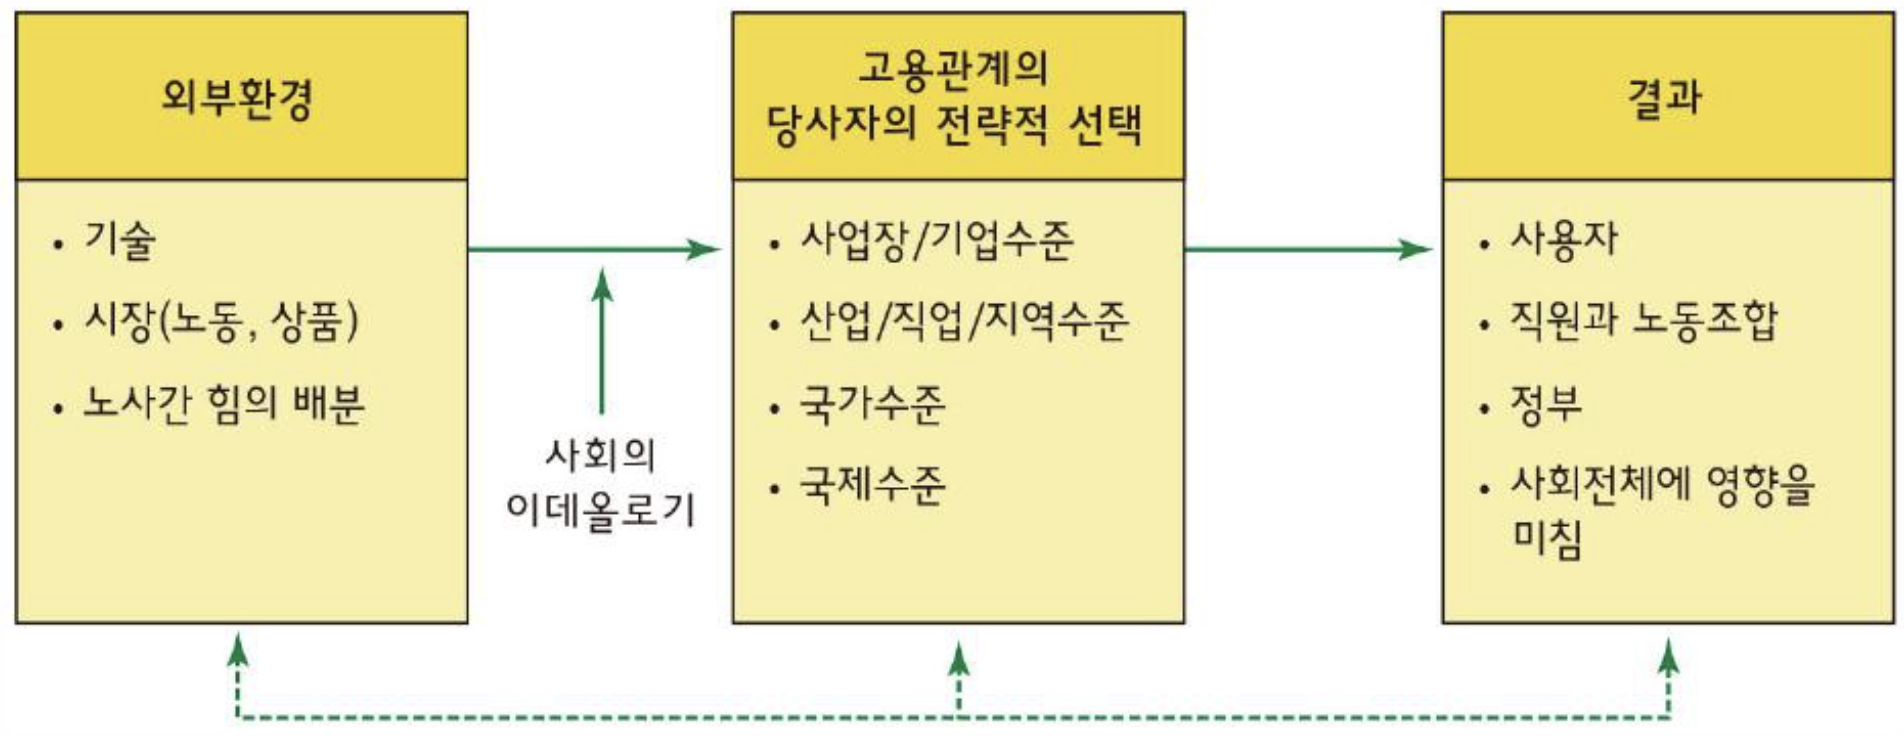
\includegraphics[width=.95\textwidth]{pic/고용관계시스템 구성.png}
        \\
        \raggedright % 왼쪽 정렬
        \hspace{1em} % 좌측 여백을 추가
        \tiny{교과서 p. 11.} % 자료 출처
        \caption{고용관계시스템의 구성}
    \end{figure}
    \begin{itemize}
        \item 
    \end{itemize}
\end{frame}

\begin{frame}
    \scriptsize
    \begin{table}
        \centering
        \resizebox{.95\textwidth}{!}{
            \centering
\begin{tabular}{|>{\centering\arraybackslash}m{2cm}|>{\centering\arraybackslash}m{2.2cm}|>{\centering\arraybackslash}m{2.2cm}|>{\centering\arraybackslash}m{2.2cm}|>{\centering\arraybackslash}m{2.2cm}|>{\centering\arraybackslash}m{2.2cm}|}
\hline
\textbf{분석수준} & \textbf{피고용인/노조} & \textbf{사용자} & \textbf{정부} & \textbf{경영의사결정} & \textbf{공동결정} \\
\hline
\textbf{사업장/기업수준} & 작업집단, 노조간부 및 노측 위원 & 노무담당, 경영자 & 노동감독관, 조정/중재위원 & 인적자원관리 전략 및 관행 & 사업장/기업수준 단체교섭 \\
\hline
\textbf{산업/직업/지역 수준} & 산별/직업별노조, 전문가 단체, 지역연대 & 사용자단체, 컨설팅회사, 노동시장 중개인 & 산업/직업 규제단체, 직업면허발급기관 & 사용자단체의 전략, 공공부문 경영 & 산별교섭 및 패턴 교섭 \\
\hline
\textbf{국가수준} & 전국단위 노조, 노동관련 사회단체 & 전국단위 사용자조직 & 정부, 법률기관 & 기업지배구조와 고용관계 영향 & 국가단위(노사정위) 교섭 및 산별교섭 결과 조정 \\
\hline
\textbf{국제수준} & 국제노동조직(연합), 노동관련 국제적 NGO & 국제사용자조직, 다국적 기업 & 범정부적 기구(EU, ILO, WTO) & 다국적기업 내 경영정책 확산 & 다국적기업의 교섭 및 협의 \\
\hline
\end{tabular}
        }
        \\
        \raggedright % 왼쪽 정렬
        \hspace{1em} % 좌측 여백을 추가
        \tiny{자료 :Paul Blyton, Edmund Heery, Nicolas Bacon, and Jack Fiorito, The SAGE Handbook of Industrial Relations, (2008), p. 7} % 자료 출처
        \caption{고용관계시스템 수준별 당사자별 활동}
    \end{table}
\end{frame}


%------------------------------------------------
\end{document}
%------------------------------------------------